Las características incluidas en este grupo describen el grado de armonicidad de la señal, es decir, su composición en términos de señales puramente armónicas.

La extracción de estos descriptores requiere la estimación de la \textbf{frecuencia fundamental} de la señal, así como de los llamados \textbf{picos armónicos} de esta.

La frecuencia fundamental ($F_0$) es la frecuencia más baja del espectro de frecuencias tal que las frecuencias dominantes en la señal pueden expresarse como múltiplos de esta.
Puede, por tanto, considerarse la $F_0$ como la frecuencia de la señal armónica que mejor representa a la señal en cuestión.

Existen numerosas variantes para la estimación de la $F_0$ de una señal~\cite{Kim05}, siendo la propuesta en~\cite{Cheveigne02} una de las más populares.
Esta técnica, también conocida como \textit{algoritmo YIN};
se basa, a grandes rasgos, en encontrar el valor del período $\tau$ que minimiza la siguiente función para cada trama $t$~\cite{Gerhard03-2}:

\begin{gather}
    \label{eq:YIN}
    d_t'(\tau) = \begin{cases}
                     1 & \tau = 0 \\
                     \frac{d_t(\tau)}{\frac{1}{\tau}{\sum_{j=1}^{\tau}{d_t(j)}}} & eoc.
    \end{cases}\\
    d_t(\tau) = \sum_{i=0}^{N-1}{(x[i]-x[i+\tau])^2}
\end{gather}

Luego, la frecuencia fundamental estará dada por la expresión $F_0 = 1/\tau$.

Conocida la frecuencia fundamental de la señal, podemos estimar sus picos armónicos, los que se localizan en torno a los múltiplos de $F_0$.
De esta forma, podemos definir el $h$-ésimo pico armónico como el valor de la DFT de la señal, localizado en la posición $k_h$ tal que:

\begin{equation}
    \label{eq:harmonicPeaks}
    k_h = \argmax_{k\in [a_h,b_h]}|X[k]|
\end{equation}

\noindent
donde los extremos del intervalo $[a_h, b_h]$ están dados por las ecuaciones:

\begin{gather*}
    a_h = \text{floor}\left[ (h - nht)\frac{F_0}{\Delta F} \right] \\
    b_h = \text{ceil}\left[ (h + nht)\frac{F_0}{\Delta F} \right]
\end{gather*}

\noindent
donde $\Delta F = F_{s}/K$ es el intervalo de frecuencias entre dos posiciones consecutivas de la DFT de la señal, $K$ es cardinalidad de la DFT;
y $nht$ es un valor denominado \textit{tolerancia no armónica}, usualmente tomado como $nht = 0.15$.

El procedimiento presentado para la estimación de los picos armónicos no siempre produce buenos resultados si las características de la señal difieren en extremo de las de una señal armónica.
Otras variantes más apropiadas para estos casos han sido diseñadas, basadas en la descomposición del proceso en dos pasos: primero la detección de \textit{picos espectrales} y luego los picos armónicos.
En esencia, se detectan todos los picos presentes en la DFT de la señal y luego se comparan con los de la señal armónica correspondiente a la frecuencia fundamental;
al final, se conservan los picos que mejor se ajusten a los de la señal armónica.~\cite{Kim05}.

\subsection{Inharmonicity}\label{subsec:inharmonicity}

La \textit{inharmonicity} (INH) representa la divergencia de las frecuencias que componen la señal respecto a los múltiplos de su frecuencia fundamental.
Se calcula mediante la expresión:

\begin{equation}
    \label{eq:INH}
    INH = \frac{2}{F_0} \frac{\sum_{h}{|f(h) - h\cdot F_0|\cdot |X[h]|^2}}{\sum_{h}{|X[h]|^2}}
\end{equation}

\noindent
donde $h$ itera por los picos armónicos de la señal, y $f(h)$ y $X[h]$ son respectivamente la frecuencia asociada al pico $h$-ésimo y el valor del coeficiente correspondiente de la DFT\@.

Los valores de la INH varían entre 0 (señal puramente armónica) y 1 (señal no armónica).

\subsection{Odd to Even Harmonic Energy Ratio}\label{subsec:oddToEvenHarmonicEnergyRatio}

Este descriptor permite distinguir entre sonidos donde predominan los múltiplos pares de la frecuencia fundamental, de aquellos donde predominan los impares, o donde ambos tienen amplitudes equivalentes.
Se computa como el cociente entre las posiciones de la DFT de la señal correspondientes a picos armónicos impares y las correspondientes a picos pares:

\begin{equation}
    OER = \frac{\sum_{h=2p+1}{|X[h]|^2}}{\sum_{h=2p}{|X[h]|^2}}, p\in\mathbb{N}\cup \{ 0 \}
\end{equation}

\subsection{Tristimulus}\label{subsec:tristimulus}

El \textit{tristimulus} (TR) fue introducido como un equivalente a los atributos de color en la visión.
Se calcula para tres conjuntos de picos armónicos, agrupados de forma equivalente al modo en que son percibidos en la audición humana.
Las fórmulas para los tres coeficientes son las siguientes:

% TODO Check this way of calling peaks with lower indices
\begin{equation}
    \begin{aligned}
        T1 & = \frac{|X[h_0]|}{\sum_{h}{|X[h]|}} \\
        T2 & = \frac{|X[h_1]|+|X[h_2]|+|X[h_3]|}{\sum_{h}{|X[h]|}} \\
        T3 & = \frac{\sum_{h\in \{h_4, h_5, \ldots, h_{H-1}\}}{|X[h]|}}{\sum_{h}{|X[h]|}}
    \end{aligned}
\end{equation}

\noindent
donde $H$ es la cantidad total de picos armónicos en la señal, y $h_i$ el pico $i$-ésimo.
El denominador es, en los tres casos, la suma de las amplitudes de las frecuencias de todos los picos armónicos.

Como se puede observar, el primer coeficiente corresponde solamente a la proporción de la energía contenida en el primer pico, $T2$ a los picos del segundo al cuarto, y $T3$ a los restantes.

\begin{figure}[!h]
    \centering
    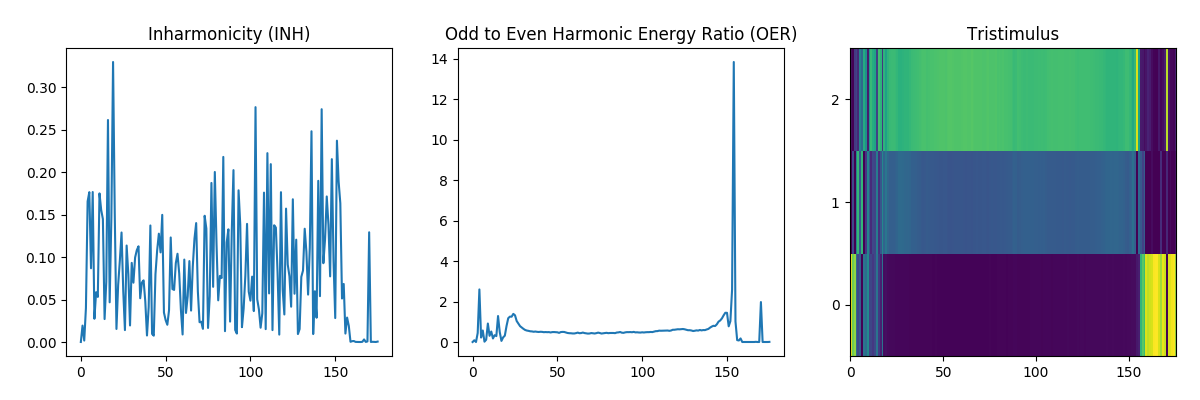
\includegraphics[width=\textwidth]{harmonic-features.png}
    \caption{Características armónicas básicas de una señal de audio.}
    \label{img:harmonic-features}
\end{figure}

\subsection{Harmonic Spectral Shape}\label{subsec:harmonicSpectralShape}

De un modo semejante al de la sección~\ref{subsec:spectralShape}, las características de este grupo describen mediante indicadores estadísticos, la representación de la señal a partir de sus picos armónicos.

\subsubsection{Harmonic Spectral Centroid}\label{subsec:harmonicSpectralCentroid}

%TODO (HSC)

\subsubsection{Harmonic Spectral Spread}\label{subsec:harmonicSpectralSpread}

%TODO (HSS)

\subsubsection{Harmonic Spectral Roll-off}\label{subsec:harmonicSpectralRoll-off}

%TODO (HSRO)


